\section{Conceptual Framework}
\label{sec:design}

\subsection{Concept}

\begin{figure}
    \centering
    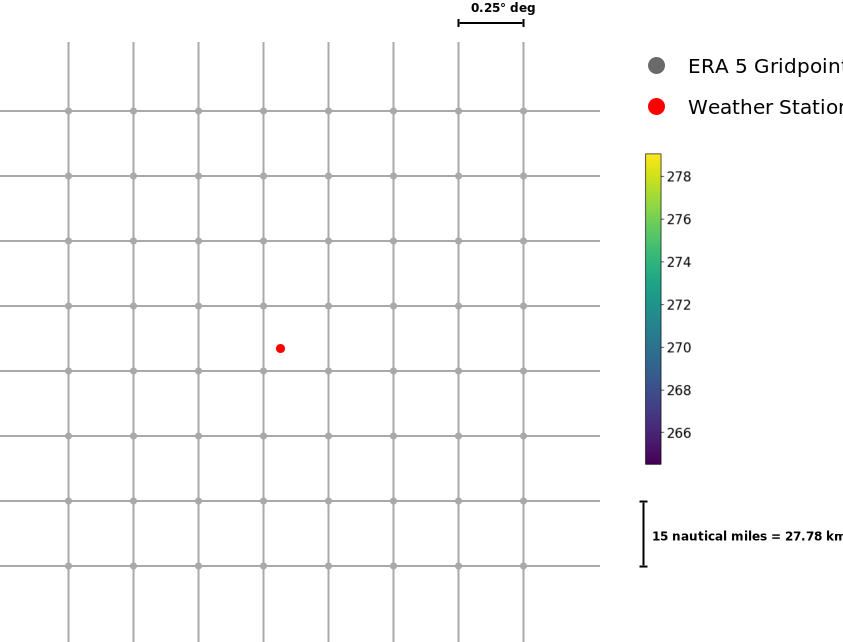
\includegraphics[width=\textwidth]{resources/images/ERA5_tas_around_barbados.png}
    \caption{8x8 grid-points of ERA5 with 2m temperature 
    for 2020-06-23 19:00 UTC  in the area of a weather station on Barbados}    
    \label{fig:barbados}
\end{figure}

\begin{figure}
    \centering
    \includegraphics[width=450pt]{resources/images/digitaltwin_schema.png}
    \caption{Conceptual Framework of the proposed method}    
    \label{fig:concept}
\end{figure}

The conceptual framework of the proposed method is illustrated in \autoref{fig:concept}. Applying the local bias of the weather station against ERA5 on top of ERA5 would reconstruct the temperature data at the station. The idea is that a Convolutional Neural Network would learn the complex behaviour of the bias depending on the arial situation, if you train it with enough available measurments. Once the CNN is trained as a model that represents the local bias of the weather station vs the ERA5 data, applying it to the ERA5 data allows for the reconstruction of missing temperature values at the weather station just by providing the data of the ERA5 temperature in the regional cutout at that timestamp used in training as an input. To illustrate what such a bias could be: In the case of Barbados for example the grid cells of the ERA5 data all lay primarly in the ocean, meaning the diurnal cycle has a much lower amplitude than at the weather station that is placed on land, the neural network would need to learn how to detect based on the 64 grid points in which phase of the diurnal cycle the weather station is and then adjust the temperature values accordingly. Besides this obvious difference between ERA5 and the measurmenets at Barbados there are most likely many more local effects to master.

Since the ERA5 data is available everywhere and for any timestep, for any hour without measurements at the weather station that the model is trained for could be reconstructed. To train the model, a supvervised learning approach would be used, meaning that the input will be ERA5 data at times where measurements are available and the expected output should be the measurements at the weather station. The model would be trained to minimize the difference between the expected output and the model's prediction through backpropagation. To allow for flexibility in application and simplicity in training, the training has to be done hour by hour, meaning the model is passed during training one timestep at a time and the weights are updated between iterations. When reconstructing missed data, hence the model is applied to the ERA5 data hour by hour as well and the result is a series of hourly predictions that are not connected in time.

% In \autoref{fig:barbados} ERA5 grid points around a weather station on Barbados are shown along with their corresponding temperature two meters above the surface. The graph is for the hour 19:00 UTC on the 23rd of June 2020. Along the latitude and longitude lines 8 grid points are selected in each dimension, such that the weather station is centered, meaning it lays between the 4th and 5th grid point in each dimension. The available longitudes and latitudes in the ERA5 model are spaced by 0.25° along the latitude and longitude from each other, which means an almost fixed distance along the latitude while the width along the longitude varies depending on how close to the poles/equator the grid points are, obviously going close to zero neat the poles. In the case of Barbados at a latitude of 13 deg the distance between 2 gridpoints along the longitude is still about 27 km.

\subsection{Data Acquisition and Preprocessing}
\label{subsec:data_preprocessing}
Upon obtaining a dataset from a weather station, it is determined where temperature data is missing. While the weather station dataset is minute-based, data could be missing only for a few minutes within an hour instead of the full hour. This would raise the question of how many missing values are acceptable to not mark the hour as missing. Sure is, that if all temperature values are missing during an hour, the hour is marked as missing.
The ERA5 data then needs to be cropped to the neighboring 8x8 grid cells, while centering the cutout as close to the weather station as possible. The available longitudes and latitudes in the ERA5 model are spaced by 0.25° along the latitude and longitude from each other, when 8x8 grid cells are selected it needs to be assured that the grid points are such selected that the coordinates of the weather station are between the 4th and 5th grid point in each dimension. 
After cropping the ERA5 dataset geographically, the data needs to be cut and divided along the time axis to match the weather station data, leading to two datasets: one with all the hours marked as missing and one with all the hours marked as present. Until the model is trained, only the dataset with all the hours marked as present will be used. 

As a result we have a dataset pair of weather station measurements and ERA5 data, that are coherant in time and space.

To determine after the training if and to which extent the model learned to reconstruct the missing data, the dataset pair is split again alogn the timeaxis into a pair of station with ERA5 data for training and oair of station with ERA5 data for validation. Thus we can later let the model reconstruct values that have actually been measured but haven't been included in the training so we then can validate how successful the reconstruction is. With the datasets prepared, the next phase involves configuring and training the Convolutional Neural Network (CNN) for the temperature reconstruction task. The CNN architecture is tailored to accept input in the form of 8x8 grid cells centered around the weather station's location. Employing a supervised learning approach, the CNN is trained using pairs of hourly temperature data from the weather station and corresponding grid cell data from ERA5. The training process iteratively feeds batches of data into the CNN, fine-tuning its parameters to minimize prediction errors and optimize accuracy in reconstructing missing temperature values.


\subsection{Model Evaluation}
Following the training phase, the CNN's performance is evaluated using the validation set. The model's capacity to accurately reconstruct missing temperature data at the weather station is scrutinized against ground truth values. This evaluation step serves to gauge the CNN's proficiency in capturing intricate weather patterns and producing precise temperature estimations. For that, the root mean squared error (RMSE) and the correlation coefficient are calculated. The RMSE is a measure of the differences between predicted and observed values, while the correlation coefficient quantifies the strength and direction of the linear relationship between the two datasets. An obvious choice as timerange for the evaluation would be to cut out one complete year so that the model can be evaluated over the full range of seasons and weather conditions. 

\subsection{Application to New Data}
Upon successful training and validation, the model is trained again with the measurements that have been exluded before in the benefit of validation. After training on the full data the CNN can be used to fill gaps. Fundamentally any list of timesteps that the model should applied for can be requested and then the ERA5 data for the respective timesteps is optained, cropped in the same way to the geographical region as before and then the model is applied to the data. The result is a list of temperature values that are not connected in time, but are the model's prediction for the temperature at the weather station at the respective time. Since in \ref{subsec:data_preprocessing} we split the ERA5 dataset already into two datasets, one with all hours marked as missing and one with all hours marked as present, the model can be applied to the dataset with all hours marked as missing and then directly infilled into the original measurements dataset.